\newcommand{\fwb}{2.3cm}
\begin{figure}
\centering
\begin{tabular}{c|c|c}
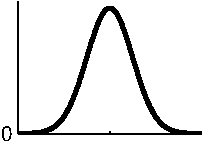
\includegraphics[width=\fwb]{../figures/structure_examples/se_kernel} &  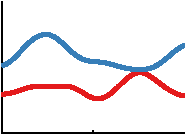
\includegraphics[width=\fwb]{../figures/structure_examples/se_kernel_draws} & 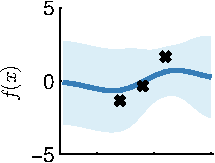
\includegraphics[width=\fwb]{../figures/structure_examples/se_kernel_post} \\
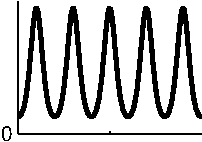
\includegraphics[width=\fwb]{../figures/structure_examples/per_kernel} &  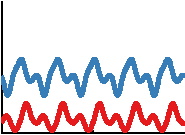
\includegraphics[width=\fwb]{../figures/structure_examples/per_kernel_draws} & 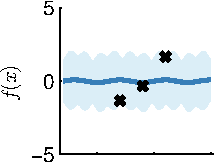
\includegraphics[width=\fwb]{../figures/structure_examples/per_kernel_post} \\
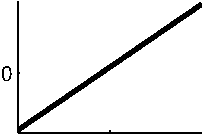
\includegraphics[width=\fwb]{../figures/structure_examples/lin_kernel} &  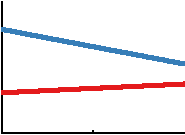
\includegraphics[width=\fwb]{../figures/structure_examples/lin_kernel_draws} & 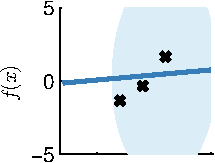
\includegraphics[width=\fwb]{../figures/structure_examples/lin_kernel_post} \\
base kernel & draws from GP & GP posterior
\end{tabular}
\caption{ Basic kernels.}
\label{fig:basic_kernels}
\end{figure}